
{\color{blue}2-4-16}

%Lattice gas
%$\La, M$ particles
%$n:\La\to \{0,1\}$
%Configuration space $\Om=\bit^{\La}$.
%Study particles within region. The fact that the total number of particles is fixed is less visible in a small region.
%For the grand canonical ensemble, we have independence.
%Can: $\Pj(n) = \fc{\one[N(n)=M]}{C}$, 
%The grand canonical ensemble $\fc{e^{-\mu N(n)}}{Z_\La(\mu)}$.
%we can compute using the entropy.
%how without stirling.
\subsection{Generalizing Ensemble Analysis to Harder Cases}

Previously we used very specific machinery to derive the grand canonical ensemble for the lattice gas; how might we derive similar expressions for more complicated systems?  We would like to avoid using the Stirling formula, which only happened to work in the simple case. 
To derive the entropy bypassing Stirling's approximation, you may proceed by analyzing partition functions. 

Define the \index{partition function}\textbf{partition function} for the grand canonical ensemble as the (unnormalized) sum of the likelihoods over all configurations. At each site there are 2 possibilities and they are independent, so the sum factors into a product.\footnote{Note that $\Lambda$ in the last section is the micro-canonical ensemble, but here it is the grand canonical ensemble.}
\begin{align}
\nonumber
Z_\Lambda & = \sum_{n\in \Omega} e^{-\mu N(n)} \\
\nonumber
&=\sum_{n\in \Omega} \prod_{x\in \Lambda} e^{-\mu \mathds{1}[n_x=1]}\\
\nonumber
&=\prod_{x\in \widetilde{\Lambda}}(1+e^{-\mu})\\
\nonumber
&= (1+e^{-\mu})^{|\Lambda|}\\
\frac{1}{|\Lambda|} \ln Z_{\Lambda} &= 1+e^{-\mu}
\label{eq:z1}\text{{\color{red}\tiny eq:z1}}
\end{align}

So what does this have to do with entropy? We can calculate $Z_\Lambda$ a different way, as follows.
Note that the only thing that matters in the summand is the number of particles in $n$, so let's group the summands by this. Letting $\rho=\frac{N}{|\Lambda|}$, and using the fact that the number of states with density $\rho$ is $e^{|\Lambda|s(\rho)}$,\footnote{Rather than getting this with $s(\rho)=-[\rho\ln(\rho) - (1-\rho) \ln (1-\rho)]$ by the Stirling approximation in the last section, we can take this as the \emph{definition} of $s$ here, and use it to solve for $s$.}
\begin{align}
\nonumber
Z_\Lambda&=\sum_{n\in \Omega} e^{-\mu N(n)}\\
\nonumber
& \approx \sum_{\rho \in \frac{1}{|\Lambda|}\mathbb{Z}} e^{-\mu N(n)} e^{|\Lambda|s(\rho)}\\
\nonumber
& =\sum_{\rho \in \frac{1}{|\Lambda|}\mathbb{Z}} e^{|\Lambda|[s(\rho)-\mu \rho]}\\
%concave modified by a linear function.
%for each $\mu$ there is some maximum.
%when you look at contribution of points $\ep$ away, it changes by a factor of the volume. 2
%all terms which are $\ep$ away contribute a negligible amount.
\label{eq:z2}\text{{\color{red}\tiny eq:z2}}
&\approx e^{|\Lambda|\max_{\rho\in [0,1]}[s(\rho)-\mu\rho]}.
\end{align}
%The multiplicity is the exponential of the volume $|\La|$ times the entropy $s(\rh)$.
%Should we should multiply by the range . 
To get the last step, note that the error we are making by focusing on the maximal point rather than counting with multiplicity the near-maximal value is at most a factor equal to the volume, since we can upper bound our error by taking all points in $\Lambda$ instead of merely an $\varepsilon$-ball around the maximum. ``In analysis, it often pays to avoid being excessively generous.'' Since $\frac{1}{|\Lambda|}\ln |\Lambda|\to 0$, this term is negligible. %details to follow
%excessively meticulous.
The expression $\max_{\rho\in [0,1]}[s(\rho)-\mu\rho]$ is called the \index{Legendre transform}\textbf{Legendre transform} of the entropy and denoted by $s^*(\rho)$. 

Matching~\eqref{eq:z1} and~\eqref{eq:z2}, we find
\be
s^*(\mu):= \max_{0\le \rho\le 1} [s(\rho) - \mu\rho] = \ln (1+e^{-\mu})
\ee
%this isn't a definition.
%can define 
%\begin{definition} Legendre entropy. \\
%\beq{eq:s-leg}
%s^*(\mu):= \max_{0\le \rh\le 1} [s(\rh) - \mu\rh] = \ln (1+e^{-\mu})
%\eeq
%\end{definition}

%The maximal value of $\fc KV$ takes it all: this is

Using this, we can derive the expression the formula for $s(\rho)$, using the inverse Legendre transform.

To check that taking the maximum in~\eqref{eq:z2} was legit, note that\footnote{Mathematicians are paranoid, so we use $\sup$ instead of $\max$. For many practical purposes they are the same.}
\begin{align*}%\llabel
\max_{\rho}[s(\rho) - \mu \rho] &\le \frac{1}{|\Lambda|}\ln Z_{\Lambda} \le \max_\rho [s(\rho)-\mu \rho] + \underbrace{\frac{1}{|\Lambda|}\ln |\Lambda|}_{\to 0}\\
\implies
\lim_{|\Lambda|\to \infty} \frac{1}{|\Lambda|}\ln Z_{\Lambda} &= \sup_{0\le \rho\le 1} [s(\rho) - \rho \mu].
\end{align*}
%We know this is true because 
%from the partition function we can extract the entropy.
%consistent with Stirling formula? Can we do without? Yes.

%comment: This is essentially the same as the series of equations~\eqref{eq:s2}.
%Now why is this equation true? It's a very fundamental point. This is true since we applied Stirling to the counting function, which comes from the fact that when you compute the partition function, it's the sum over all allowed configurations: $Z_N = \sum_{m \in \Omega} e^{-\mu N(m)}$. Let's classify these terms according to the value of $N$. Recall density $\rho$ is just number of particles per volume: $N/ |\Lambda|$. Let's write $N(m) = \rho\cdot |\Lambda|$. Thus we can rewrite $Z_N = \sum_{\rho_{1/|\Lambda|}} e^{-\mu \rho |\Lambda|}e^{|\Lambda|s(\rho)} = \sum_{\rho_{1/|\Lambda|}} e^{|\Lambda|(s(\rho) - \mu \rho)}$. $\rho \in [0, 1]$ and we discretize over $1/|\Lambda|$. As we saw before, we use the maximum because when we deviate a small amount from the maximum, a \textbf{slight drop}, all terms which are $\epsilon$ away, contribute an entirely negligible amount. 
%Hence 
%\be
%\max_{0\le \rh\le 1}[s(\rh) - \mu\rh] = 1+e^{-\mu}
%\ee
%This is essentially Legendre transform. It is in particular invertible.
%Stirling's approximation gave us the answer for the entropy. Any other model: you will not have the luxury of the Stirling approx argument. 

We can verify that  $s(\rho) = -[\rho\ln \rho +(1-\rho) \ln (1-\rho)]$
does indeed make~\eqref{eq:s-leg} hold. We find the maximum (critical point) or $s(\rho)-\mu \rho$ by setting the derivative to 0.\footnote{Don't differentiate in public.} 
We use the trick 
\be[x(\ln x-1)]'=\ln x.\ee We can subtract 1 from each of the logs changing the expression by a constant. Thus
\be
s'(\rho) = -\ln \rho +\ln (1-\rho) - \mu \implies \frac{\rho}{1-\rho}=e^{-\mu}.
\ee
We can use this to solve for $\rho$ and find $s^*(\mu)$ (do this yourself).
%Solving gives $\fc{\rh}{1-\rh}=e^{-\mu}$. 

In general, a micro-canonical ensemble specifies all the conserved quantities: Particles, energies, and whatever else there is. The grand canonical ensemble also generalizes by changing the factor to $e^{-\mu N} e^{\beta H}$.
Such factors are referred to as \index{Gibbs factors}\textbf{Gibbs factors} %states
or Gibbs measures.
%variational characterization of those.
%Our next topics are:
%\begin{itemize}
%\item
%Legendre transform
%\item
%Convexity/concavity
%\item A variational characterization of Gibbs states
%\item First order phase transitions (thermodynamics and statistical mechanics perspectives)
%\end{itemize}

\section{Concavity and the Legendre transform}

\subsection{Basic concavity results}

\begin{definition}
A function on $\mathbb{R}^k$ is \index{concave}\textbf{concave} if for any $x_0,x_1\in \mathbb{R}^k$, $0\le \lambda \le 1$,
\be
F(\lambda x_1+(1-\lambda)x_0)\geq \lambda F(x_1)+(1-\lambda) F(x_0).
\ee
For a \index{convex}\textbf{convex} function, the same inequality with the sign flipped holds. A negative convex function is concave. 
Concavity (convexity) means if you draw a chord between two points, it will lie below (above) the curve.\footnote{``As Richard Feynmann pointed out, getting the sign right is the hardest thing.''}
\end{definition}
%A concave curve frowns.

%useful for variational principle
For a strictly concave function, a maximum, whenever it exists, is unique.
%Feynman: getting the sign right is the hardest thing.

\begin{theorem}
For any concave function on $\mathbb{R}$, 
\begin{enumerate}
\item
The directional derivatives $F'(x\pm0)$ exist at all $x\in \mathbb{R}$. The \index{directional derivative}\textbf{directional derivative} is defined as
\begin{align*}
F'(x+0)&=\lim_{\varepsilon\to 0^+} \frac{F(x+\varepsilon)-F(x)}{\varepsilon}\\
F'(x-0)&=\lim_{\varepsilon\to 0^-} \frac{F(x+\varepsilon)-F(x)}{\varepsilon}.
\end{align*}
\item $F'(x-0)\ge F'(x+0)$ and $F'(x\pm 0)$ are decreasing.
\item For all but countably many values $x\in \mathbb{R}$, $F'(x-0)=F'(x+0)$, i.e., $F$ is differentiable at $x$.
\item Let $F_n$ be a sequence of concave functions which converge pointwise: for all $x$, $\lim_{N\to \infty} F_N(x)=:\widetilde{F}(x)$ exists. 
Then
\begin{enumerate}
\item
 $\widetilde{F}$ is concave.
\item
At points of differentiability of $\widetilde{F}$, the derivatives also converge,\footnote{Finite energy functions are always smooth, but %as a baby's face
their limit can have discontinuous derivative.
%Converge pointwise without derivative converging.
}
\be
F'(x\pm 0) \to \widetilde{F}'(x).
\ee
\end{enumerate}
\end{enumerate}
\end{theorem}

\begin{center}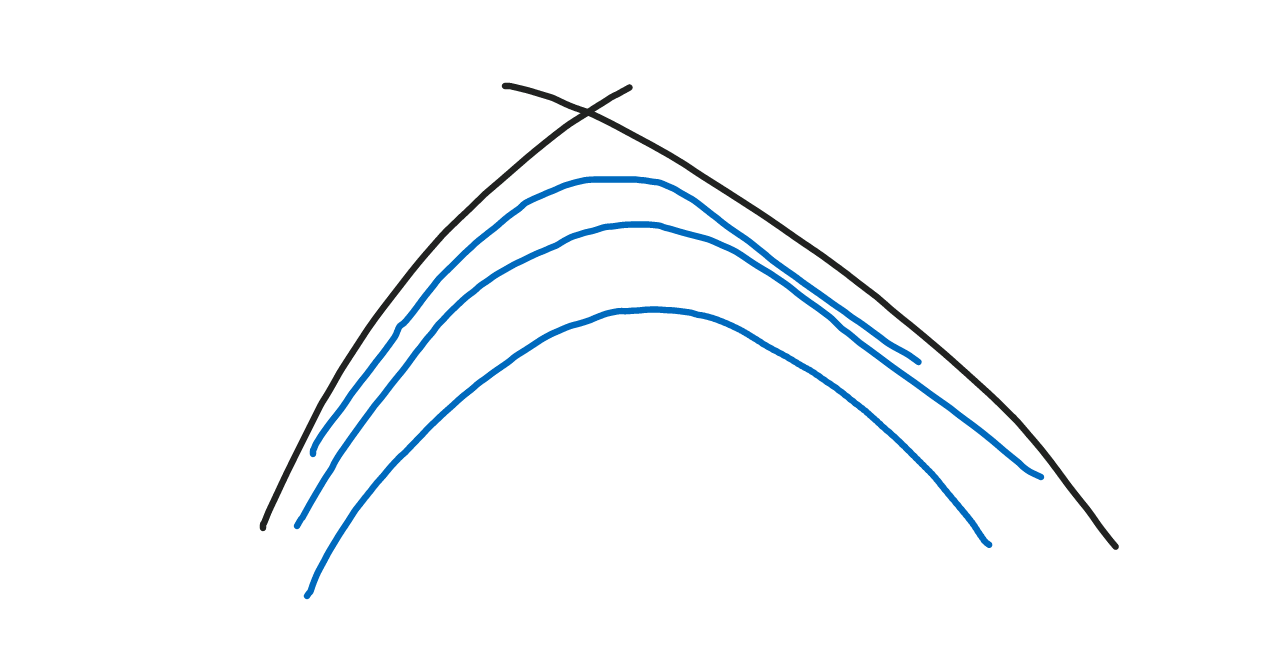
\includegraphics[scale=.25]{images/2-3}\end{center}

Much of this generalizes to directional derivatives in $n$ dimensions.
\begin{proof}
For (1) note that concavity implies that the slope of the line between $x,x+\varepsilon$ is increasing as $\varepsilon\to 0^+$.

\begin{center}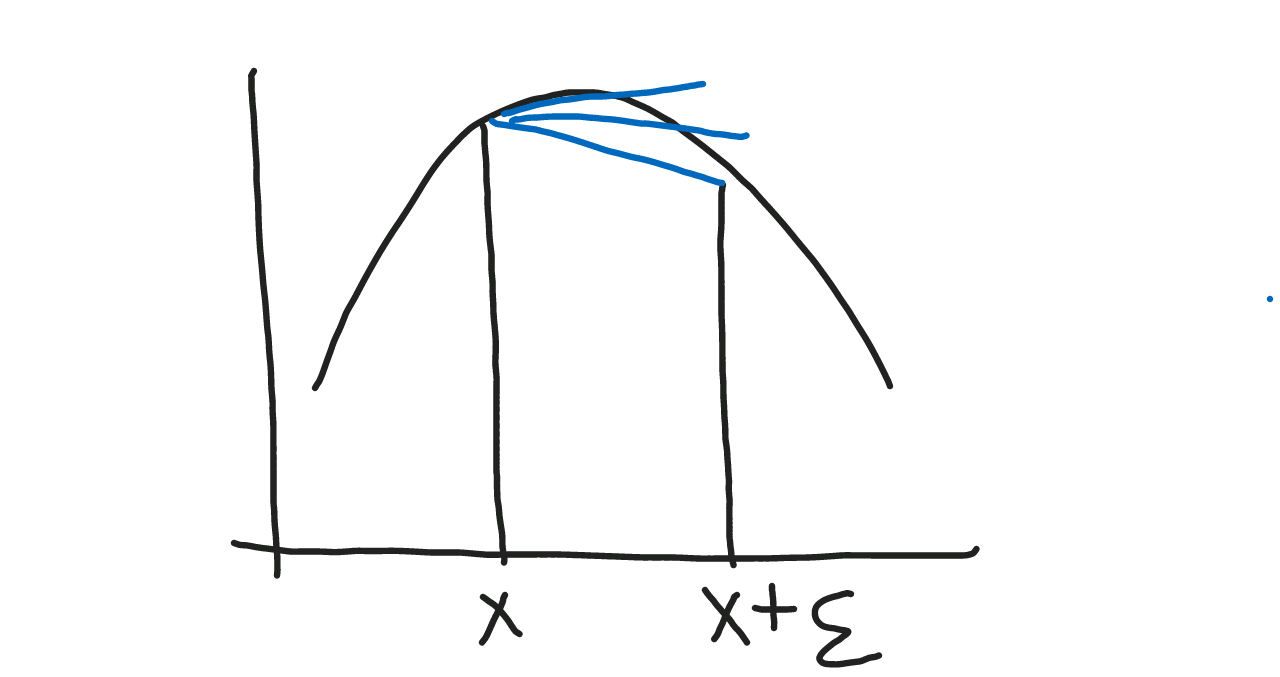
\includegraphics[scale=.25]{images/2-1}\end{center}

%The slope of the line between $x,x-\ep$ is decreasing as $\ep\to 0^-$.
To prove (3), consider the graph of the derivative $F'(x + 0)$. It's a monotone decreasing function: it starts somewhere and goes down. 
%Rewrite
At points where $F'(x+0)$ is continuous, we have $F'(x+0)=F'(x-0)$. The discontinuities, or ``steps," are the points where $F'(x+0)\ne F'(x-0)$. Now we use the fact that the sum of any uncountable collection of nonzero numbers is $\infty$. 
Applying this to the steps, we find that the number of steps is countable, i.e., the total collection of discontinuity points has to be countable.\footnote{More rigorously, for every nonzero interval $[F'(x+0),F'(x-0)]$, we can associate with it a rational number. Then note $\mathbb{Q}$ is countable.}
%Hence, if you have a function which decreases by steps, the total collection of discontinuity points has to be countable.
%It may actually decrease by steps. A nice thing about monotone steps is that a sum of any uncountable collection of nonzero numbers is $\infty$.\footnote{More rigorously, for every nonzero interval $[F'(x+0),F'(x-0)]$, we can associate with it a rational number. Then note $\Q$ is countable. } If you have a function which decreases by steps, the total collection of discontinuity points has to be countable. %The total sum of the drops is finite, which implies that the number of drops is actually finite. 
%This is FALSE: it can be countable.
%At points where there is a continuity, they agree. They only disagree at points of discontinuity. Since we have summable jumps, the collection of points of discontinuity is at most countable.
\footnote{The set of discontinuities can still be devilishly dense, ex. all the rational numbers. In physics it used to be thought that weird functions with Cantor-like sets of discontinuties could not occur, but there are materials whose free energy discontinuities are dense in certain areas.}

\begin{center}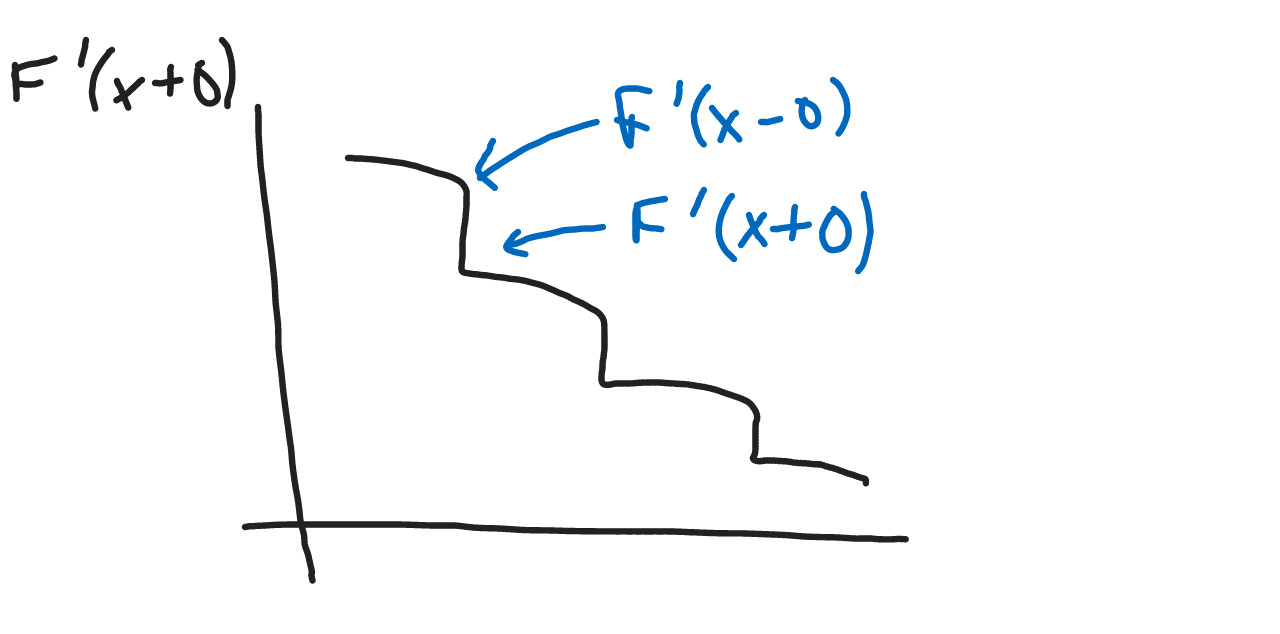
\includegraphics[scale=.25]{images/2-2}\end{center}
\end{proof}

\subsection{Concave properties of the Legendre transform}

\begin{definition}
The \index{Legendre transform}\textbf{Legendre transform} of a function is defined as
\be
(TG)(y) = \inf_x [y\cdot x - G(x)] = - \sup_x [G(x) - y\cdot x]
\ee
\end{definition}
\begin{theorem}
For any function $G$, $TG$ is concave.
\end{theorem}
%You can futz with $\ep$, but from a certain angle this is immediate.
\begin{proof}
An efficient way to think about this is the following: for each value of the parameter $x$, as a function of $y$ this is a linear function. For each $x$ we get a linear function. Define the transform by taking the infimum over that. 

Take 2 points and draw the chord between them. For each linear function the chord lies below it.\footnote{I.e., we use the following : Let $\mathcal{F}$ be a collection of concave (e.g. linear) functions. Then $\inf_{f\in \mathcal{F}}f(x)$ is concave.} 

\begin{center}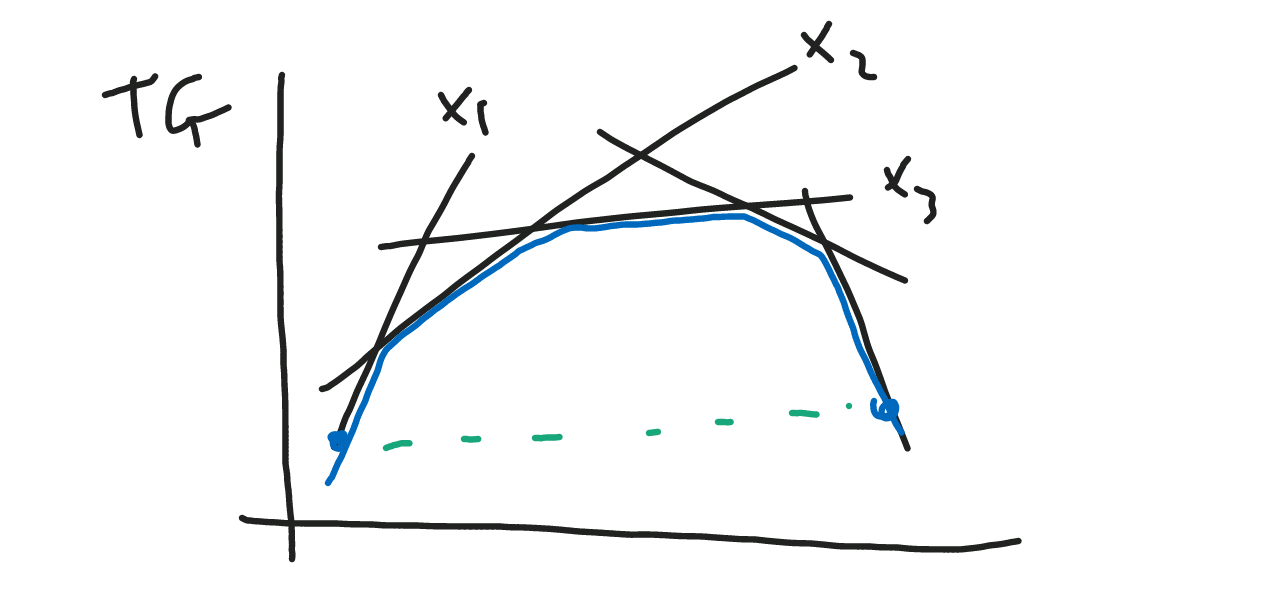
\includegraphics[scale=.25]{images/2-4}\end{center}
\end{proof}
\begin{definition}
The \index{concave hull}\textbf{concave hull} $\widetilde{G}$ of $G$ is defined as the smallest concave function that is at least the function value at every point:
\be
\widetilde{G}(x)=\inf \left\{{F(x)}:{F\text{ concave, }\forall u, \,F(u)\ge G(u)}\right\}.
\ee
%look at all functions that are concave and dominate it.
\end{definition}

\begin{center}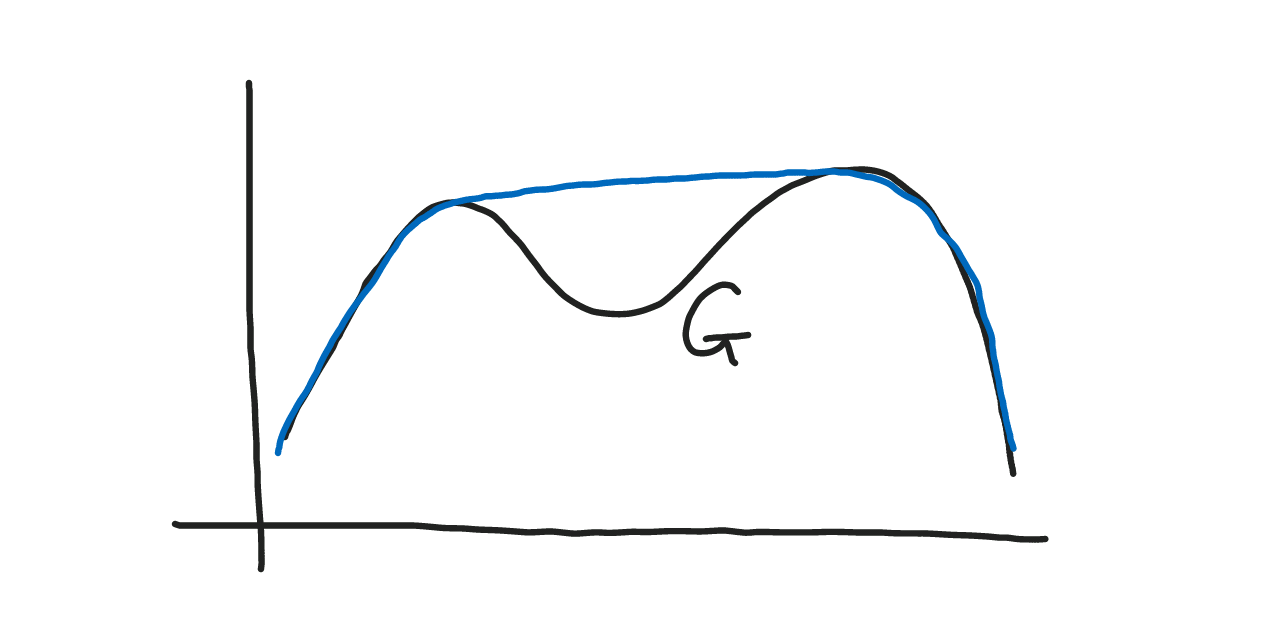
\includegraphics[scale=.25]{images/2-5}\end{center}

\begin{theorem}
For \emph{concave} $G$,
\be
T(TG)=G.
\ee
In general, $T(TG)$ is the concave hull of $G$. 
\end{theorem}
\begin{proof}[Proof for $G$ differentiable]
Use the fact that if $G$ is differentiable, then
\be
\inf_x [y\cdot x - G(x)]
\ee
occurs at $y=G'(x)$. %learn about function in discontinuous fashion. exactly what happens in 1st order phase transitions.
\end{proof}

Note that we plotted the function and the dual function on the same graph. However, they have inverse units, for example, energy and inverse temperature. You get a lot of insights into physics if you keep track of the units.
%energy and inverse temperature. You get a lot of insights into physics if you keep track of the units. Note $x,y$ have inverse units.


Recall $\rho=\frac{N}{|\Lambda|}$. %prob within configurations of observing something.
If all $2^{|\Lambda|}$ configurations are given equal weight, the typical value or $\rho$, the particles per unit volume is $\frac{1}{2}$. The Law of Large Numbers says that with probability 1 the ratio tends to $\frac{1}{2}$. Is it possible that the density is $\frac{1}{3}$? Yes, but the probability of such a density is given by the entropy: it's exponentially small, $e^{|\Lambda|[s\left( {\frac{1}{3}} \right) -\ln 2]}$. Anything other than $\frac{1}{2}$ is a large deviation; they occur with exponentially small probability. We want to quantify the probability of large deviation events. Here is a language that people found useful.
\begin{definition}\label{df:ldp}\text{{\color{red}\tiny df:ldp}}
A sequence of probability measures on $\mathbb{R}$ is said to satisfy a \index{large deviation principle}\textbf{large deviation principle} with speed $\{a_N\}$, and rate function $I(x)$ if for each $x\in \mathbb{R}$, $\varepsilon>0$,
%raghu vadhan
\be
-\inf_{|u-x|<\varepsilon} I(u)\le 
\varliminf_{N\to \infty}\frac{1}{a_N} \ln \mathbb{P}_N((x-\varepsilon,x+\varepsilon]) \le \varlimsup_{N\to \infty} \frac{1}{a_N} \ln \mathbb{P}_N((x-\varepsilon,x+\varepsilon]) \le 
-\inf_{|x-u|\le \varepsilon} I(u)
\ee
%much more complicated situations
\end{definition}
For us, $I(x)=\ln 2 - s(x)$.
%This definition generalizes the situation where the previous applies.

